% Values and vector precision/recall curves are copied from the full test run.
\begin{frame}{Cooperation Improves Detection}
  \SlideBody{\begin{VisualCanvas}
    \node[anchor=north,inner sep=0pt,text=MoverNavy,
      font=\fontsize{11}{13}\selectfont] at (7.4,5.66) {%
      \renewcommand{\arraystretch}{1.00}
      \begin{tabular}{@{}lcc@{}}
        \toprule
        \makebox[6.1cm][l]{\textbf{Condition}} &
        \makebox[3.25cm]{\textbf{AP@0.5 (\%)}} &
        \makebox[3.25cm]{\textbf{AP@0.7 (\%)}} \\
        \midrule
        Own Scan Only & 49.10 & 43.05 \\
        \textbf{Cooperative Perception} & \textbf{70.41} & \textbf{64.82} \\
        \bottomrule
      \end{tabular}};
    \node[inner sep=0pt] at (7.4,2.00)
      {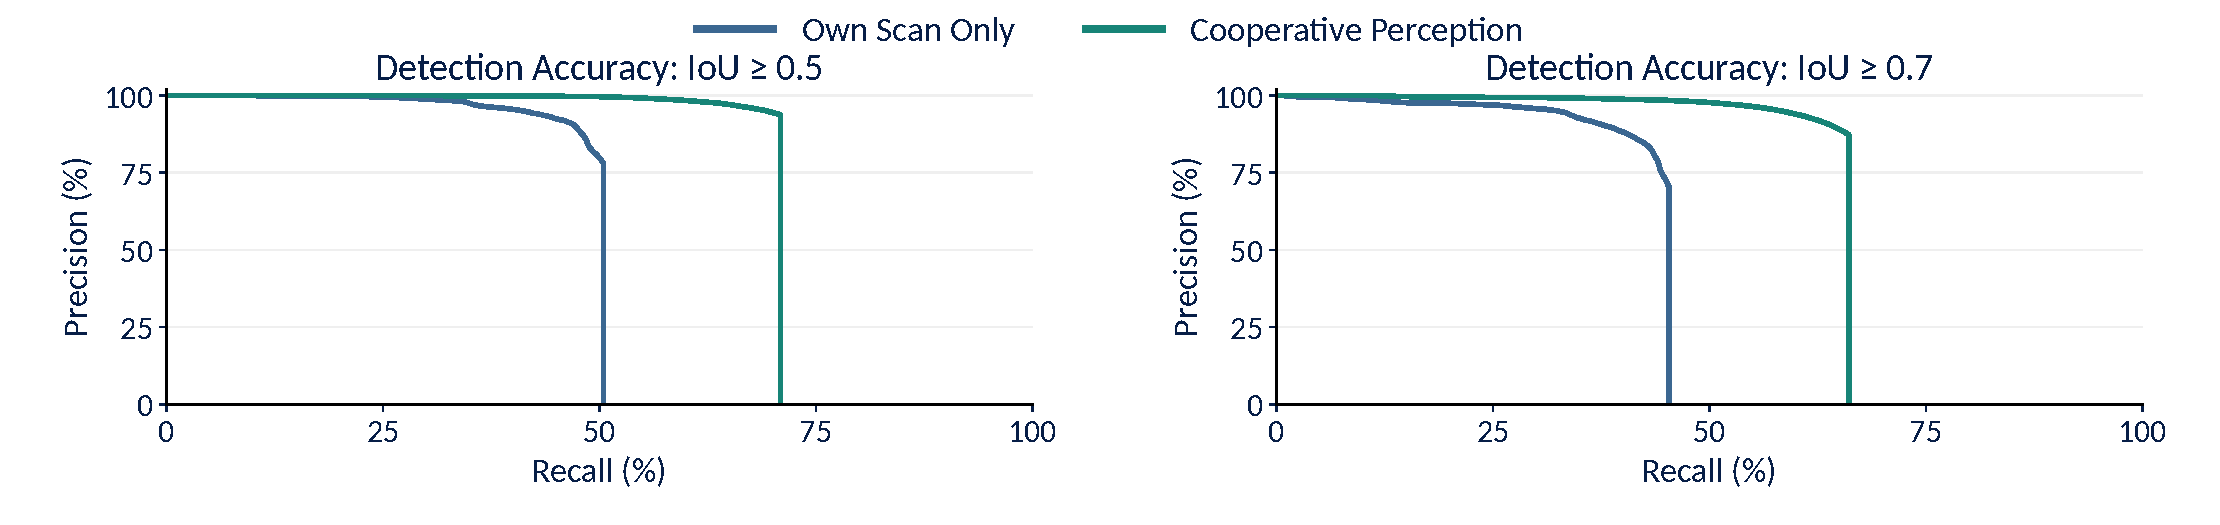
\includegraphics[width=14.4cm,height=3.45cm,keepaspectratio]{assets/experiments/w45-2026-11-04/results-plots-v1.pdf}};
    \node[final caption,font=\bfseries\fontsize{12}{15}\selectfont]
      at (7.4,0.15) {Sharing Adds 21.31 / 21.77 AP Percentage Points};
  \end{VisualCanvas}}
  \SlideSource{Source: Li et al., DiscoNet (method).}
\end{frame}
